% ============================================================
%  04.2  Build Process — Team 0109D  (ESC204 Design Dossier)
%  Helvetica 12 pt  |  0.5 in margins  |  2 pages
% ============================================================
\documentclass[12pt]{article}

% ----- Fonts & Encoding ---------------------------------
\usepackage[T1]{fontenc}
\usepackage{helvet}
\renewcommand{\familydefault}{\sfdefault}

% ----- Page Geometry ------------------------------------
\usepackage[
  letterpaper,
  margin=0.5in
]{geometry}

% ----- Packages -----------------------------------------
\usepackage{graphicx}
\graphicspath{{../images/}}
\usepackage{booktabs}
\usepackage{tabularx}
\usepackage{enumitem}
\usepackage{caption}
\usepackage{subcaption}
\usepackage{listings}
\usepackage{xcolor}
\usepackage{float}
\usepackage{parskip}

% ----- Listings Style -----------------------------------
\lstdefinestyle{pystyle}{
  language=Python,
  basicstyle=\ttfamily\scriptsize,
  keywordstyle=\bfseries\color[rgb]{0.0,0.0,0.6},
  commentstyle=\itshape\color[rgb]{0.4,0.4,0.4},
  stringstyle=\color[rgb]{0.6,0.0,0.0},
  showstringspaces=false,
  frame=single,
  framesep=3pt,
  xleftmargin=6pt,
  xrightmargin=6pt,
  aboveskip=4pt,
  belowskip=2pt,
  numbers=left,
  numberstyle=\tiny\color{gray},
  numbersep=5pt,
  breaklines=true,
}

% ----- Compact spacing ----------------------------------
\setlist{nosep, leftmargin=1.2em}
\setlength{\parskip}{3pt plus 1pt minus 1pt}
\setlength{\parindent}{0pt}
\setlength{\abovecaptionskip}{3pt}
\setlength{\belowcaptionskip}{1pt}
\setlength{\floatsep}{4pt plus 1pt minus 1pt}
\setlength{\textfloatsep}{4pt plus 1pt minus 1pt}
\setlength{\intextsep}{4pt plus 1pt minus 1pt}

% ----- Section formatting -------------------------------
\usepackage{titlesec}
\titleformat{\section}{\large\bfseries}{}{0em}{}
\titlespacing*{\section}{0pt}{6pt}{2pt}
\titleformat{\subsection}{\normalsize\bfseries}{}{0em}{}
\titlespacing*{\subsection}{0pt}{4pt}{1pt}

% ========================================================
\begin{document}

% ----- Title Block --------------------------------------
\begin{center}
  {\LARGE\bfseries Subsystem Build Process}\\[2pt]
  {\large Team 0109D --- ESC204 Design Dossier}
\end{center}

\vspace{1pt}
\hrule
\vspace{4pt}

% ========================================================
\section{1\quad Electrical Subsystem Build}
% ========================================================

Three design iterations converged on the final production-ready configuration.

\begin{table}[H]
\centering
\small
\begin{tabularx}{\textwidth}{@{}l l X l@{}}
\toprule
\textbf{Iteration} & \textbf{Motor / Driver} & \textbf{Outcome} & \textbf{Power} \\
\midrule
V1 & DC motor, breadboard     & Functional but imprecise; no position control & 9\,V battery \\
V2 & DC motor, L298N H-Bridge & Failed --- voltage drop across L298N left insufficient torque & 9\,V battery \\
Final & Nema\,17 stepper, A4988 driver, screw-terminal blocks & Full position control; reliable operation & 12\,V DC adapter \\
\bottomrule
\end{tabularx}
\caption{Circuit iteration summary.}
\end{table}

% --- Iteration photos (side-by-side) --------------------
\begin{figure}[H]
\centering
\begin{subfigure}[t]{0.30\textwidth}
  \centering
  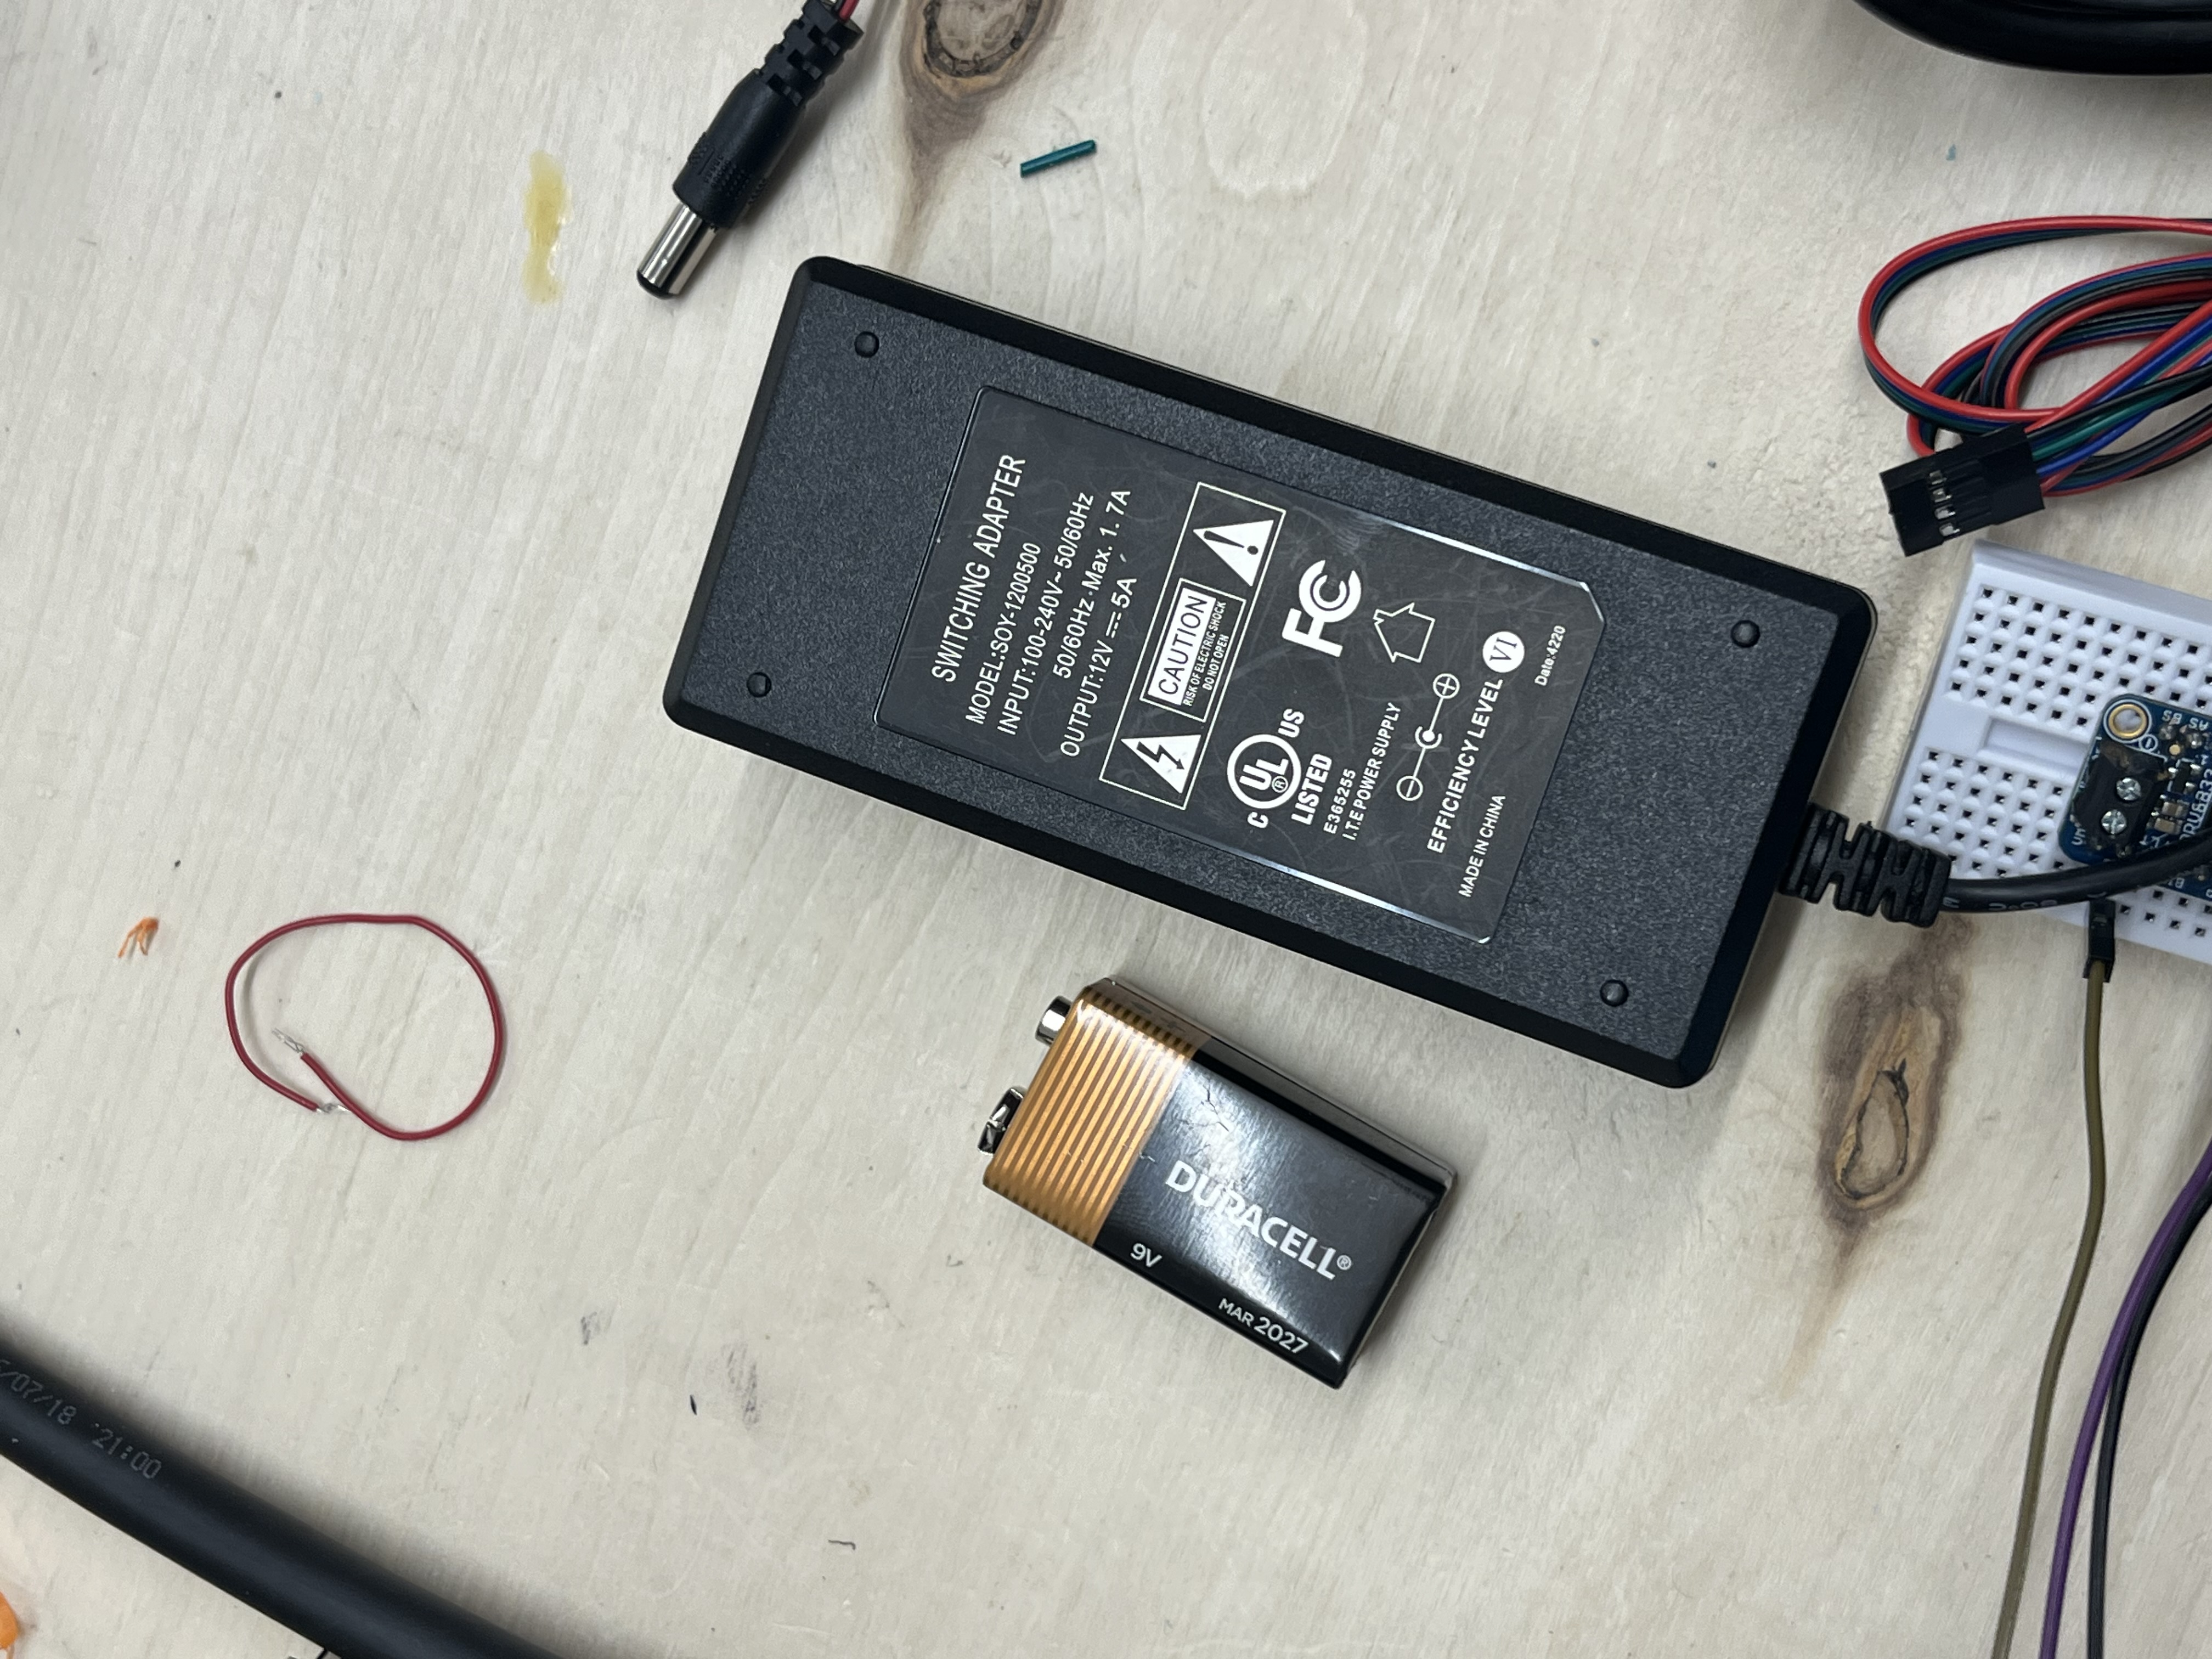
\includegraphics[width=\linewidth,height=3.2cm,keepaspectratio]{DC_Motor_Breadboard_Iteration1.jpeg}
  \caption{V1 --- DC motor on breadboard.}
\end{subfigure}\hfill
\begin{subfigure}[t]{0.30\textwidth}
  \centering
  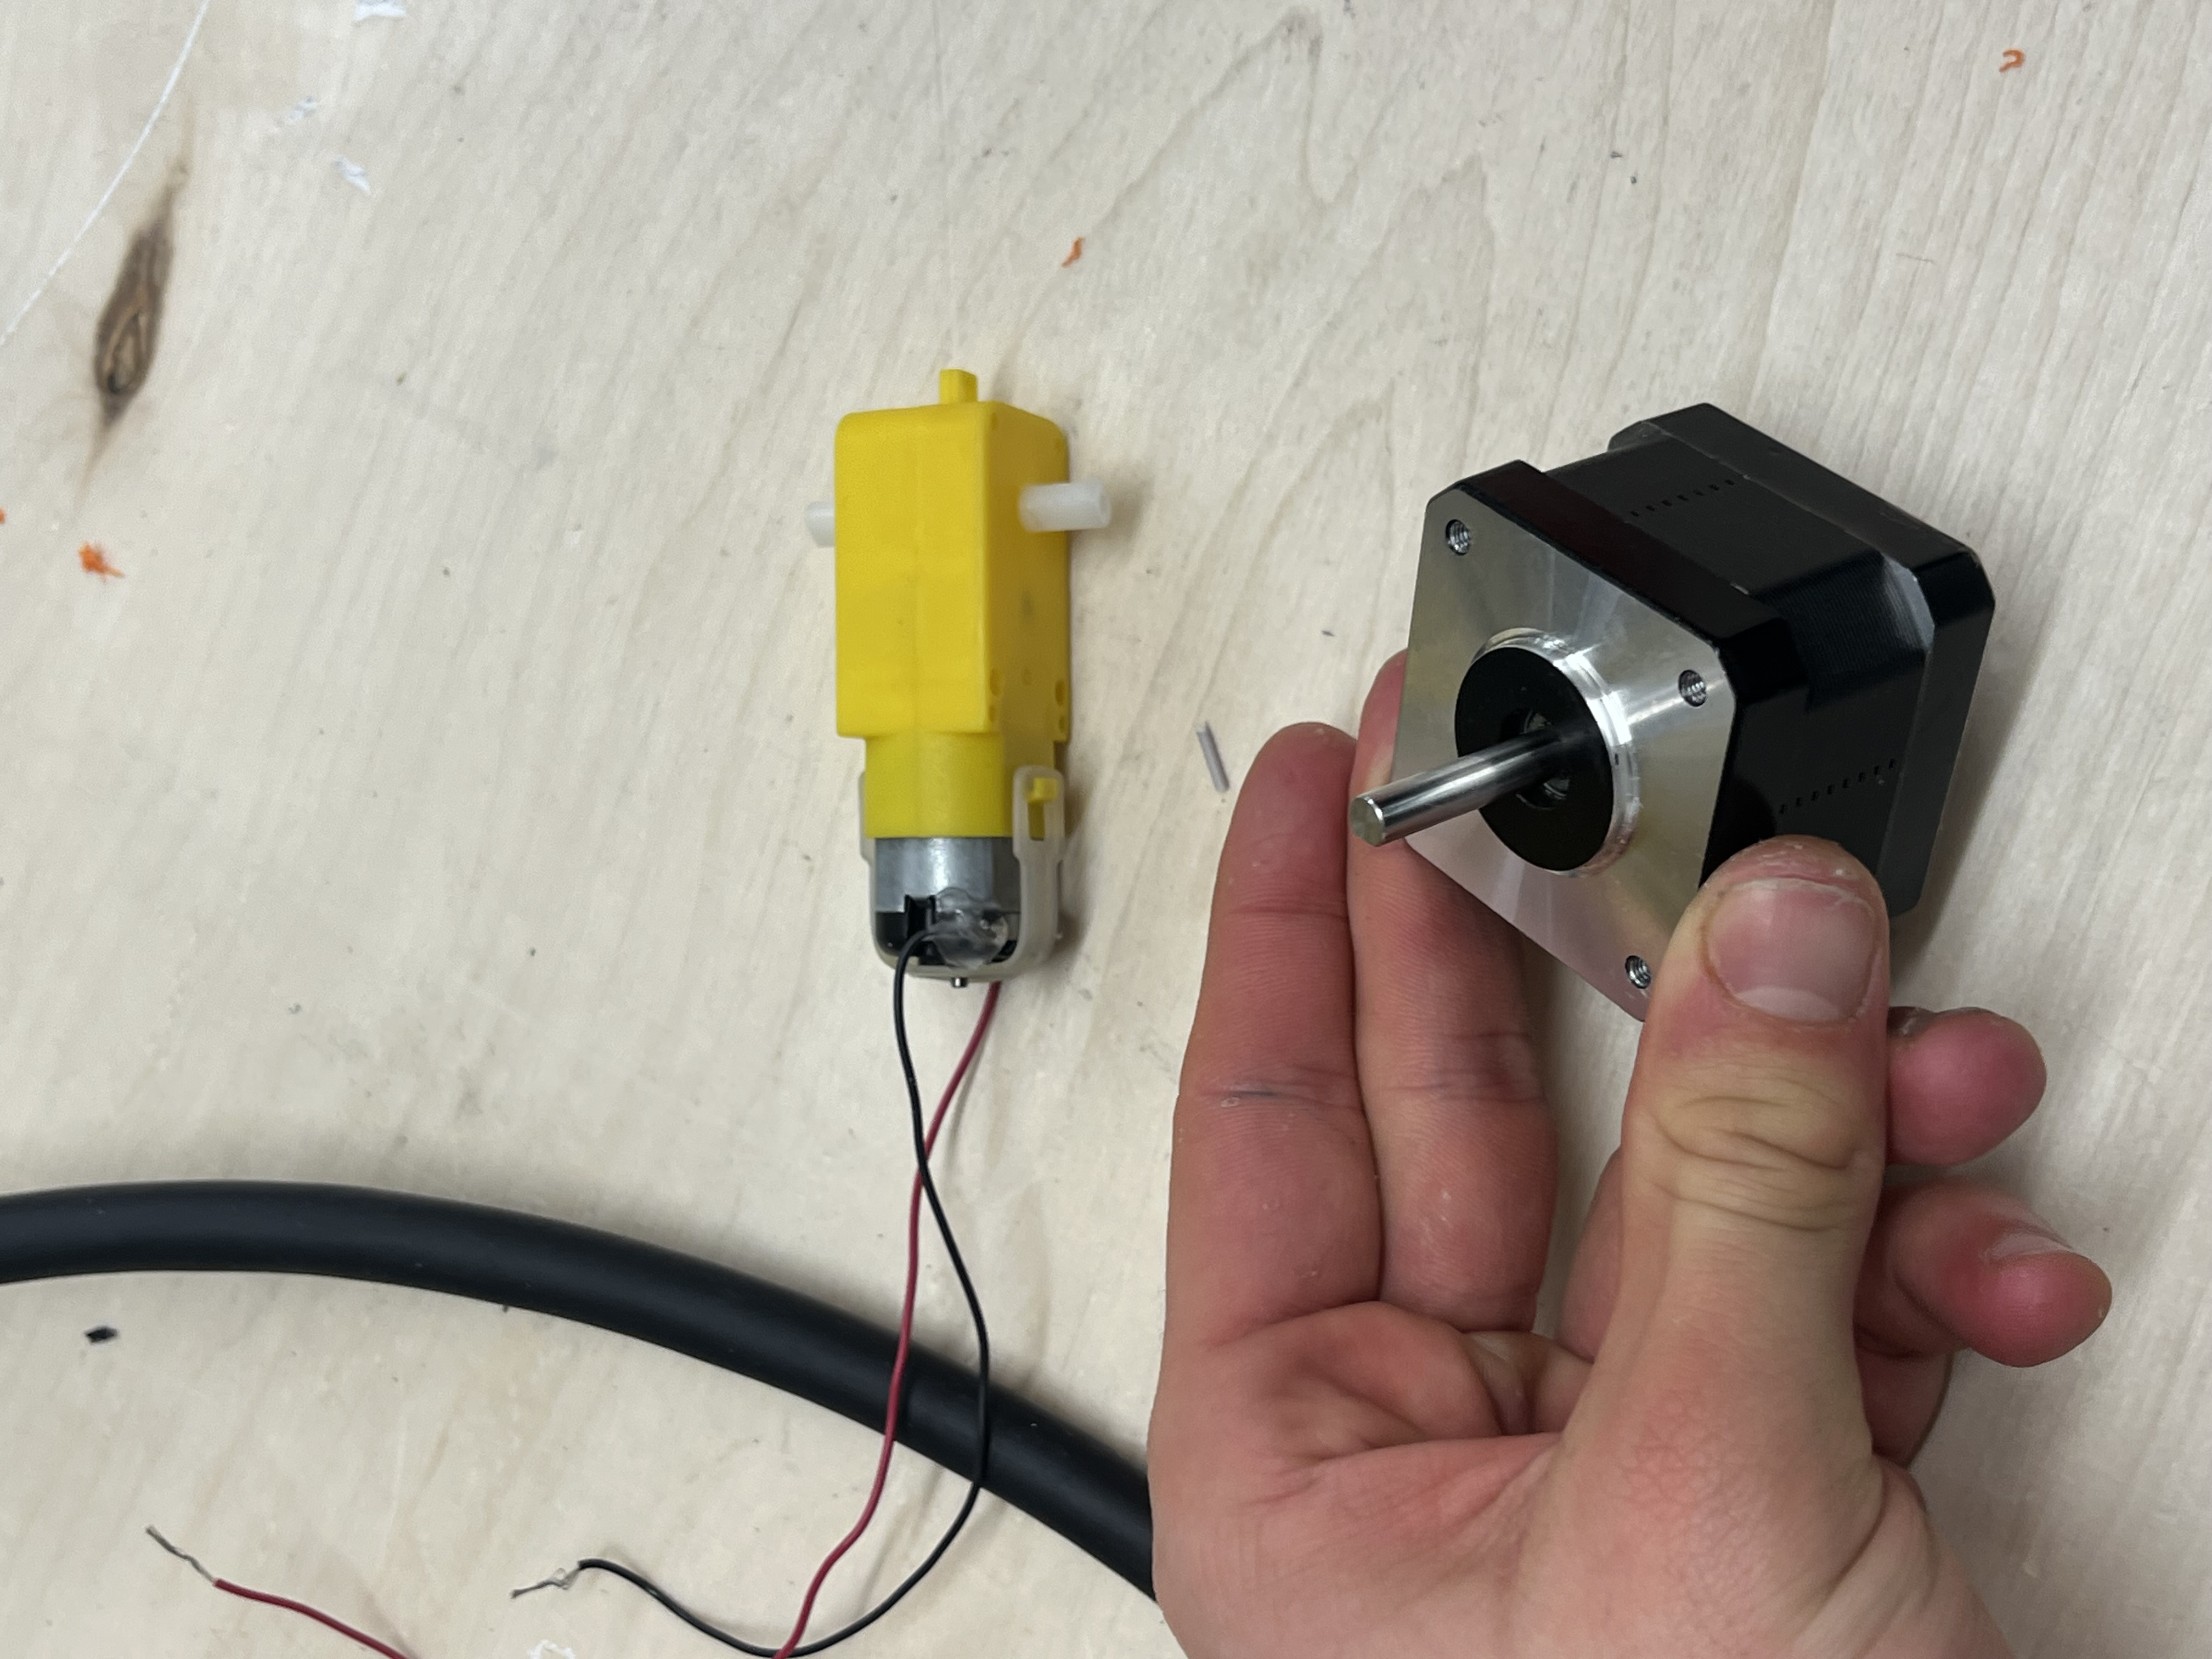
\includegraphics[width=\linewidth,height=3.2cm,keepaspectratio]{HBridge_Motor_Iteration2.jpeg}
  \caption{V2 --- L298N H-Bridge.}
\end{subfigure}\hfill
\begin{subfigure}[t]{0.30\textwidth}
  \centering
  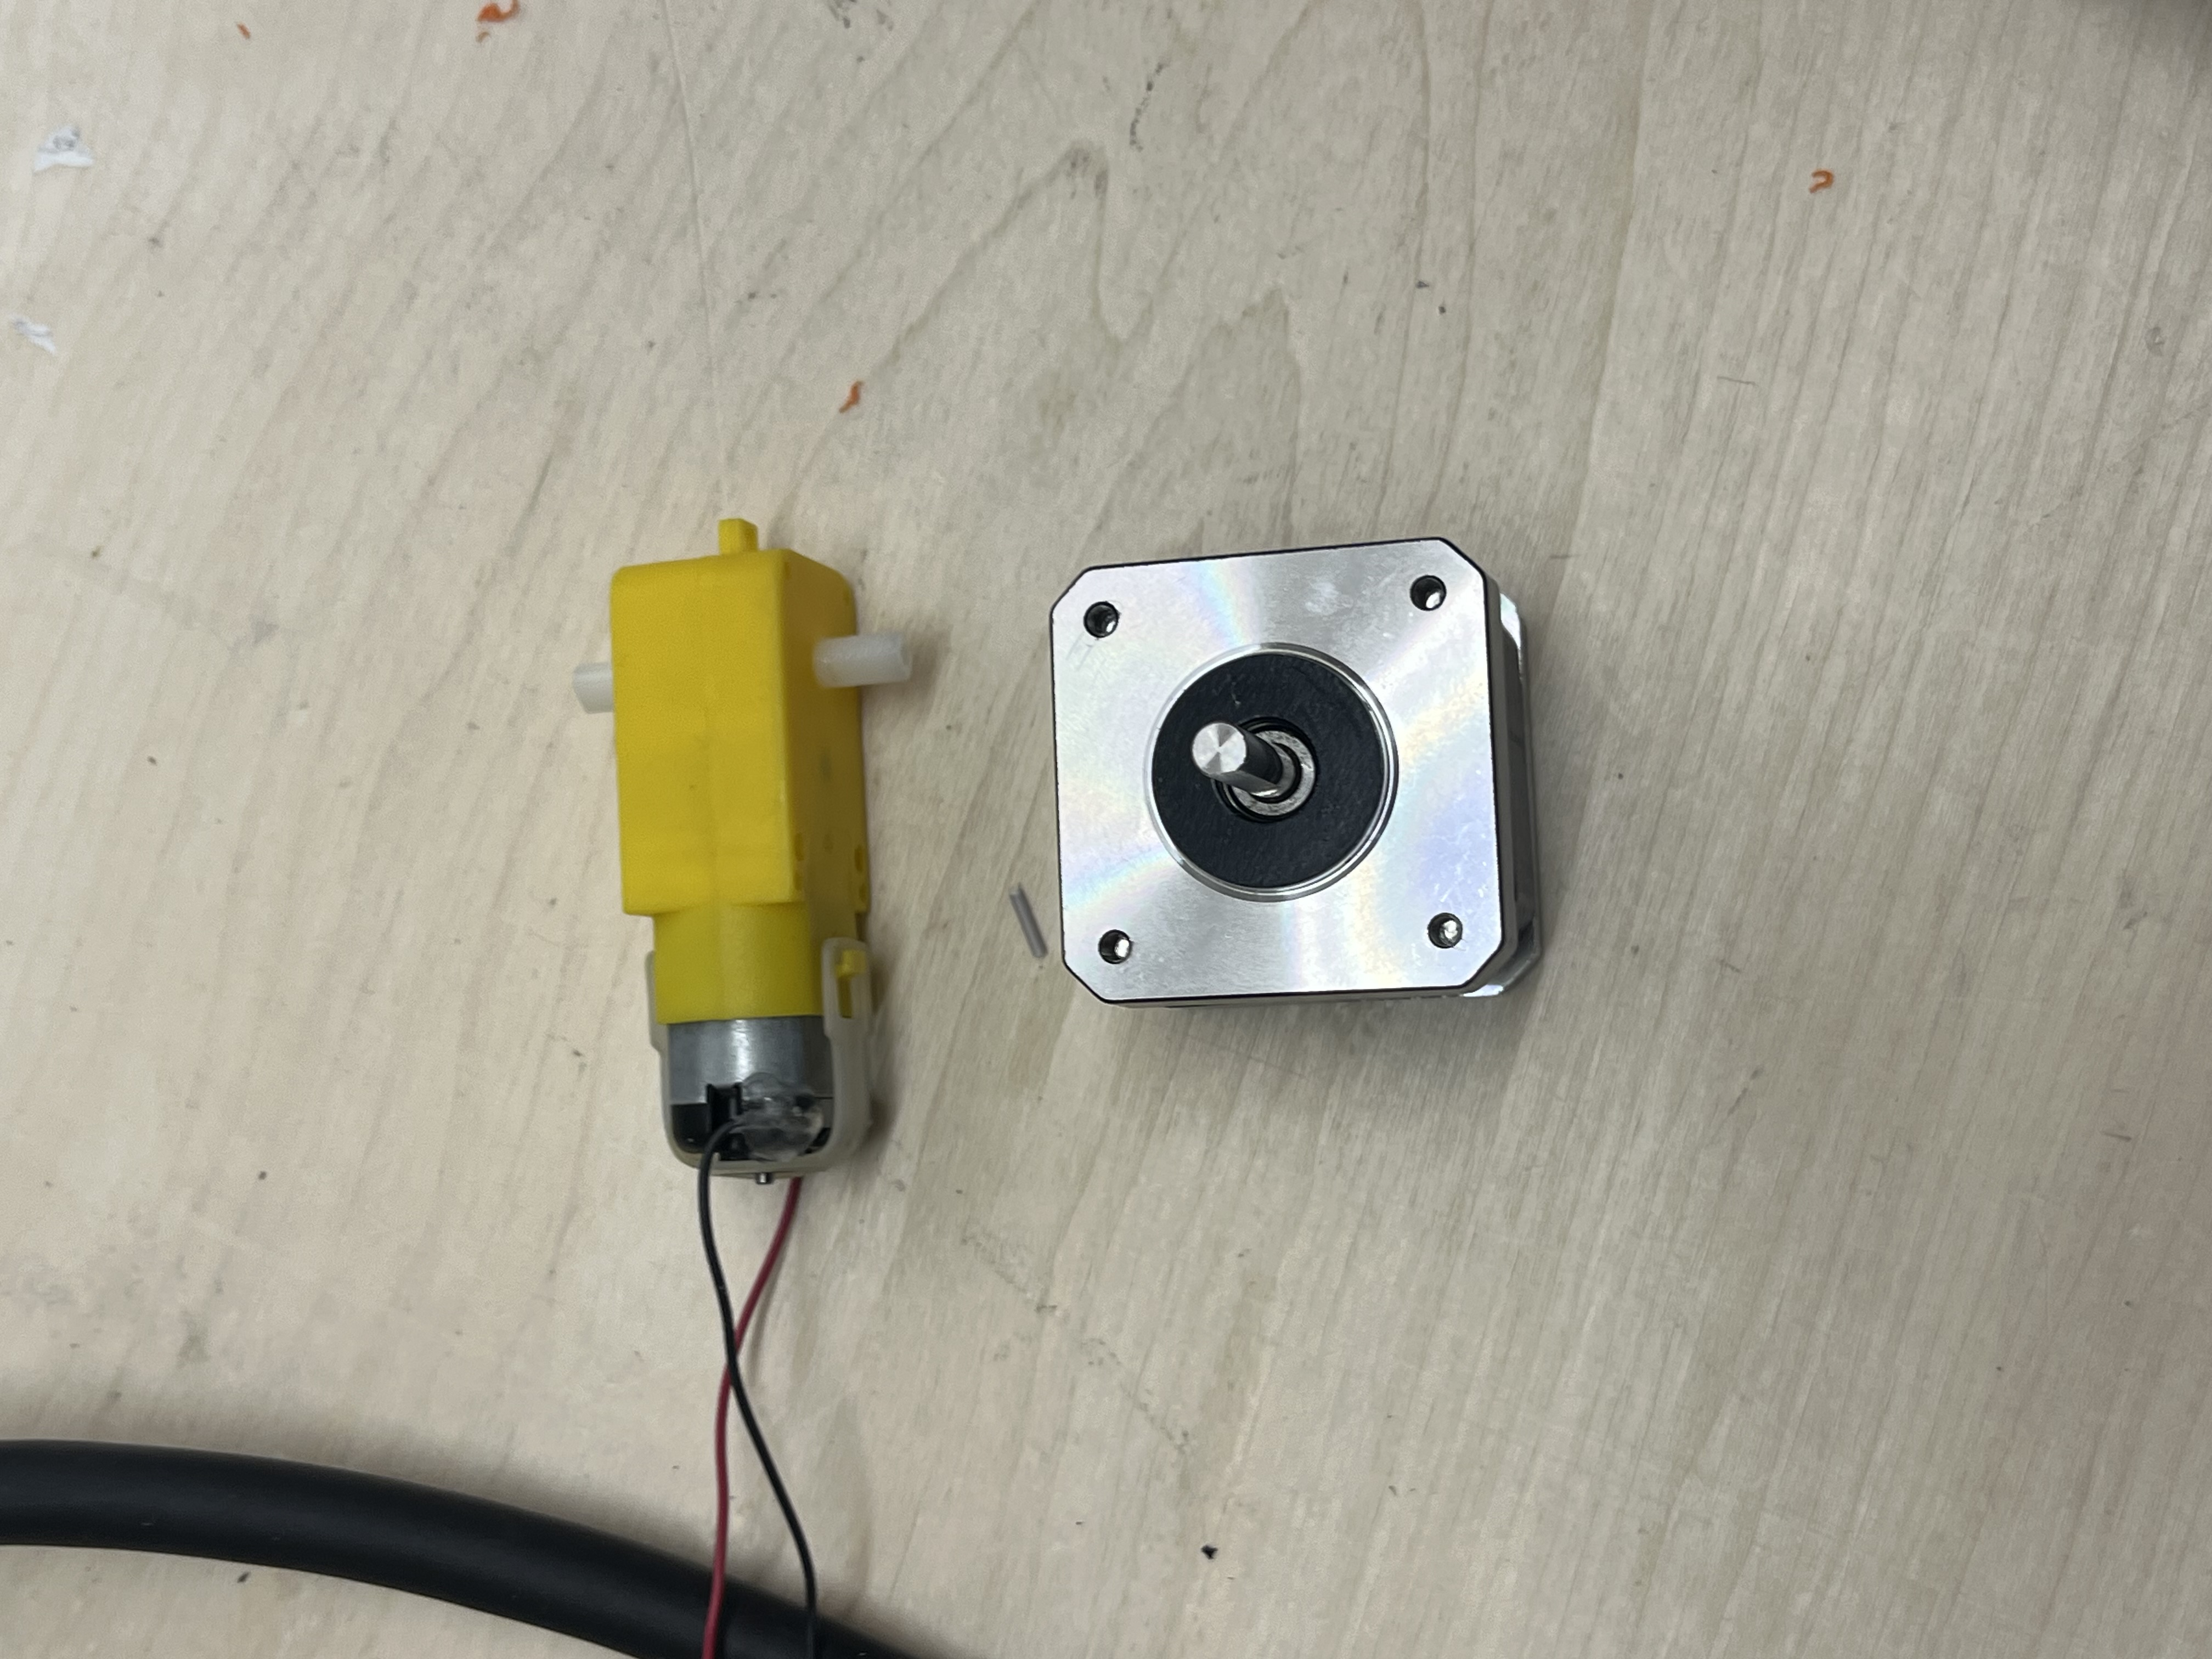
\includegraphics[width=\linewidth,height=3.2cm,keepaspectratio]{Stepper_A4988_ScrewTerminals_Final.jpeg}
  \caption{Final --- A4988 + screw terminals.}
\end{subfigure}
\caption{Electrical subsystem iterations (V1 $\rightarrow$ V2 $\rightarrow$ Final).}
\end{figure}

\subsection{Wiring Layout}
Derived from \texttt{firmware/code.py}:

\begin{table}[H]
\centering
\small
\begin{tabular}{@{}l l l@{}}
\toprule
\textbf{Signal} & \textbf{Pin} & \textbf{Notes} \\
\midrule
A4988 STEP  & GP2 & Pulse line \\
A4988 DIR   & GP3 & Direction select \\
A4988 EN    & GP4 & LOW = enabled \\
Limit SW Home (NO) & GP5 & Internal PULL\_UP; wired to GND \\
Limit SW End (NO)  & GP6 & Internal PULL\_UP; wired to GND \\
\bottomrule
\end{tabular}
\caption{Pico GPIO wiring map.}
\end{table}

\textbf{Power isolation:} 5\,V USB supplies Pico logic; a separate 12\,V DC adapter powers the A4988 VMOT rail. No motor current flows through the Pico ground path.

% ========================================================
\section{2\quad Mechanical Subsystem Build}
% ========================================================

\textbf{Ridge Track:} 60\,cm aluminum T-slot extrusion (purchased from MYFab
catalogue) provides a rigid, low-friction rail.

\subsection{Pulley System Iterations}

\begin{table}[H]
\centering
\small
\begin{tabularx}{\textwidth}{@{}l X X@{}}
\toprule
\textbf{Aspect} & \textbf{V1} & \textbf{V2 (Final)} \\
\midrule
Axles       & Thin --- teardrop cross-section (FDM artifact) & Thicker --- true circular cross-section \\
Brackets    & L-shaped; bent under belt tension               & Triangle-reinforced; rigid under load \\
Belt        & Smooth TPU; slipped under load                  & TPU with molded grip indents \\
\bottomrule
\end{tabularx}
\caption{Pulley system iteration comparison.}
\end{table}

\textbf{Final belt specification:} GT2 timing belt, 2\,mm pitch, mated to a
20-tooth pulley giving \textbf{40\,mm per revolution} (200 full-steps/rev
$\Rightarrow$ 0.2\,mm/step).  Total track allows \textbf{56\,cm active travel}
between the two limit switches.

% ========================================================
\section{3\quad Software Subsystem Build}
% ========================================================

\textbf{Platform:} Raspberry Pi Pico running CircuitPython.

\textbf{Architecture:} Reactive state machine polling limit switches, accepting single-character serial commands:

\begin{table}[H]
\centering
\small
\begin{tabular}{@{}c l@{}}
\toprule
\textbf{Command} & \textbf{Action} \\
\midrule
\texttt{H} & Home --- drive backward until home switch triggers, zero position \\
\texttt{F} & Full pass --- traverse home $\rightarrow$ end $\rightarrow$ home \\
\texttt{M} & Move forward 100\,mm \\
\texttt{B} & Move backward 100\,mm \\
\bottomrule
\end{tabular}
\caption{Serial command set.}
\end{table}

\textbf{Key parameters:}
\texttt{STEP\_DELAY\_S}\,=\,0.0008\,s ($\approx$625\,steps/s),\quad
\texttt{MM\_PER\_STEP}\,=\,0.2\,mm.

\subsection{Limit-Switch Guard (from \texttt{single\_step()})}

The guard checks the relevant limit switch \emph{before} pulsing STEP, preventing cart overrun:

\begin{lstlisting}[style=pystyle]
def single_step(direction):
    """Pulse STEP once with limit-switch guard. Returns True if step taken."""
    if direction == DIR_FORWARD and end_pressed():
        return False
    if direction == DIR_BACKWARD and home_pressed():
        return False

    pin_step.value = True
    time.sleep(0.000005)
    pin_step.value = False
    time.sleep(STEP_DELAY_S)

    global current_step_position
    current_step_position += 1 if direction == DIR_FORWARD else -1
    return True
\end{lstlisting}

% ========================================================
\section{4\quad Fabrication Methods}
% ========================================================

\begin{table}[H]
\centering
\small
\begin{tabularx}{\textwidth}{@{}l l X@{}}
\toprule
\textbf{Method} & \textbf{Facility} & \textbf{Components Produced} \\
\midrule
FDM 3D Printing (PLA) & MYFab & Pulleys, axles, brackets, nozzle cart \\
FDM 3D Printing (TPU) & MYFab & Timing belt with molded grip indents \\
Purchased Stock        & MYFab Catalogue & 60\,cm aluminum T-slot extrusion \\
Soldering              & Lab & Wire connections to limit switches and A4988 screw terminals \\
\bottomrule
\end{tabularx}
\caption{Fabrication method summary.}
\end{table}

All 3D-printed parts were fabricated at MYFab. TPU belt printing required reduced speed (20\,mm/s) and direct-drive extrusion for dimensional accuracy on grip indents. Soldered joints were heat-shrink sleeved for strain relief.

\end{document}
